\chapter{The ALICE TPC Upgrade} \label{ch:tpcu}

From 2014 until 2018, I worked on the upgrade of the TPC to a continuous readout.  This included working on a test beam in 2014 for a prototype Read-Out Chamber (ROC) using Micropattern Gaseous Detectors (MPGD) over the current Multi-Wire Proportional Chamber (MWPC) design.  Once a final design for the new ROCs was chosen the production of the new Inner Read-Out Chambers (IROCs) using a stack of four Gaseous Electron Multiplier (GEM) foils took place at the University of Tennessee.  During this period I assembled 49 new IROCs.  In 2018, I traveled to Yale University and CERN to help with quality assurance of the IROCs built at Tennessee.


\section{Physics Motivation}
As of the end of 2018, the LHC has been in the second long shutdown (LS2) and upgrading to the High Luminosity LHC (Hi-Lumi LHC)\cite{Apollinari:2015bam} which was briefly mentioned in Section \ref{sec:LHC}.  The goal of the LHC upgrade is to move into an era of high precision measurements of rare QCD processes and increase the production of soft probes.  Once the upgrade is complete the expected event rate in ALICE will be 50 kHz in MinBias PbPb collisions.  This will lead to a factor of x100 increase in MinBias data and a factor of x10 increase in high-$p_{T}$ triggered data recorded by ALICE.

The ALICE experiment has focused on probing the thermodynamic properties of the QGP in the past.  The increase in event rate expected from the Hi-Lumi LHC will open new ways to probe the QGP including\cite{Abelev:1475243}:

\begin{itemize}
\item Increasing the production of jets and allowing separation of jet measurements based on the flavor of the initial parton.
\item Studying the production mechanisms of light-nuclei, antihyper-nuclei, and other exotic hadrons.
\item Probing the initial state of the QGP by measuring low-mass dileptons that originate from the earliest stages of a heavy-ion collision.
\item Increasing the yields of heavy-flavor mesons reconstructed via secondary-vertices. 
\end{itemize}

\noindent
In order to do this ALICE will implement a number of upgrades \cite{1742-6596-589-1-012014} during the shutdown that include:

\begin{itemize}
\item Replacing the V0 and T0 detectors with a combined detector, called the Forward Interaction Trigger (FIT)\cite{1742-6596-798-1-012186}.
\item Improving the ITS and Muon Tracker spatial resolution by using  Monolithic Active Pixel Sensors (MAPS)\cite{Abelev:1625842}\cite{CERN-LHCC-2015-001}.
\item Removing the 400 nanosecond dead time associated with the TPC and upgrading the FEE cards to handle the increase in data bandwidth\cite{Abelev:1475243}.
\item Implementing new Online/Offline ($O^{2}$) data processing architecture\cite{Buncic:2011297}.
\end{itemize}

Leptons weakly couple to the QGP\cite{Ryblewski:2015sha} and by studying these the initial states in heavy ion collisions may be probed\cite{Mauricio:2007vz}.  Figure \ref{fig:lowmassdilep} on the left shows a simulation of the mass spectra for dileptons between 0 GeV/\textit{c} - 1 GeV/\textit{c} using the current ALICE central detectors with tight kinematic cuts.  The yields that are quantifiable do not allow for the separation of leptons created via different processes in the QGP.  After the increase in event rate and the upgraded ITS with improved tracking capabilities, measuring the low-mass dileptons that interacted with the QGP will be possible as shown on the right of Figure \ref{fig:lowmassdilep}. 

\begin{figure}[h]
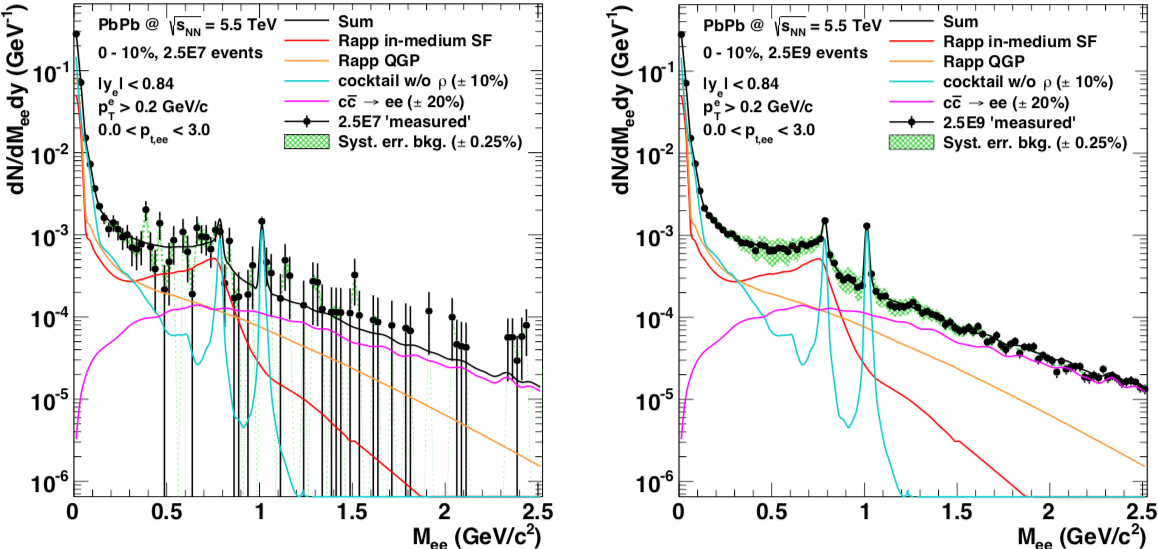
\includegraphics[width=\linewidth]{dilepton-mass}
\centering
\caption{Simulation of the invariant  mass spectra for dileptons in a typical heavy-ion run with current ALICE performance (left) and after upgrade of ALICE for Run-3 (right) in PbPb at $\sqrt{s_{NN}}$ = 5.5 TeV.  The dilepton yields originating from the QGP are shown (red and orange), along with background contributions from light-hadrons (blue), and charm (magenta)\cite{Abelev:1475243}.}
\label{fig:lowmassdilep}
\end{figure}


The TPC used in the ALICE experiment along with the readout was discussed in Section \ref{sec:tpc}.  The ALICE collaboration first proposed an upgrade of the TPC in 2012 with a Letter of Intent (LoI)\cite{Abelev:1475243}.  A Technical Design Report (TDR)\cite{CERN-LHCC-2013-020} was published in 2013 with an initial design overview.  An addendum to the TDR\cite{CERN-LHCC-2015-002} was published in 2015 after the performance of prototype ROCs was measured on a test beam at CERN in 2014.  The overall goals of the TPC upgrade are to continuously readout events in the high luminosity environment expected after LS2, to minimize the accumulation of space-charge distortions in the drift field, and to maintain the PID and tracking performance of the current TPC.


\section{Gaseous Electron Multiplier Foils}
Gaseous Electron Multiplier (GEM) Foils were first proposed by CERN physicist Fabio Sauli in 1997\cite{Sauli:1997qp}.  GEMs belong to a new form of detector technology known as Micropattern Gaseous Detectors\cite{Titov:2013hmq} that use microelectronic or chemical etching techniques to print a readout structure onto a material surface.

\begin{figure}[h]
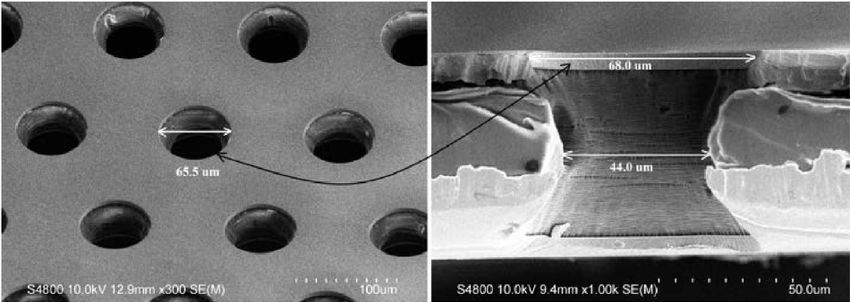
\includegraphics[width=14.0cm]{Scanning-electron-microscopy-image-of-GEM-foil-top-view-left-and-cross-section-right}
\centering
\caption{Scanning electron microscope image of a GEM foil from top (left) and profile (right)\cite{Brucken:2017qjy}.}
\label{fig:GEMpic}
\end{figure}

GEM foils are a Kapton sheet, typically 50 $\mu m$ thick, with a thin copper coat on both sides of the surface.  A weak acid and stencil are used to chemically etch holes throughout the foil.  Typically, the holes are between 10 $\mu m$ - 100 $\mu m$ in diameter and between 100 $\mu m$ - 300 $\mu m$ in pitch, as seen in Figure \ref{fig:GEMpic}.  A few hundred volts is applied to each of the copper surfaces of the GEM foil causing a strong electric field to be induced in the GEM holes\footnote{The electric field is on the order of 10 kV/cm}.  

When an ionization electron from a charged track enters a GEM hole it will cause an avalanche of electrons and ions to be produced, amplifying the signal, to MWPCs.  Due to the high voltage and strong electric fields around the GEM foil, any back flow ions created from the avalanche will get absorbed by the copper surfaces on the GEM foil, as seen in Figure \ref{fig:GEMefield}.
\begin{figure}[h]
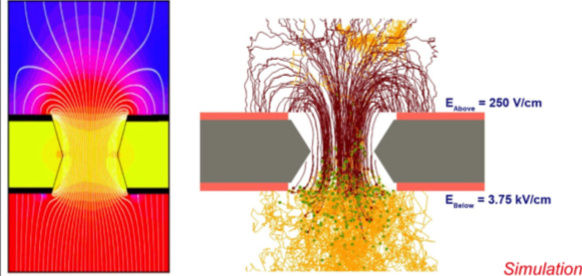
\includegraphics[width=14.0cm]{ALICEGEMSIMULATION}
\centering
\caption{Profile of GEM with electric-field lines and gradients (left).  Simulation of an ionization electron (yellow line) entering a GEM from a drift volume, amplification electrons (green dots, yellow lines) and back flow ions (red lines) are created (right)\cite{Bhattacharya:2017yaj}.}
\label{fig:GEMefield}
\end{figure}

The configuration of the pitch and size of the holes on a GEM foil is directly correlated to the amplification properties and ability to capture back flow ions.  GEMs with larger holes or shorter pitch between the holes will have more amplification but will also be more ineffective at capturing ions.  Likewise, GEMs with shorter holes or larger pitch will have better ion capturing abilities yet worse amplification properties.  By stacking multiple GEMs on top of one another it is possible to maximize the amplification properties and minimize the backflow. 

Creating GEMs with a uniform hole distribution and stacking them in a consistent manner in order to minimize the overlap of holes from one layer to another restricted them to small prototypes and impeded their use on large experiments.  Around 2010 two methods were developed, the single-mask technique\cite{0960-1317-17-8-021} and the NS2 assembly\cite{1748-0221-12-06-C06036}, which allowed for a systematic way of etching holes and stretching GEMs so they could be properly aligned.  These methods allowed for GEMs to become a viable amplification device for large experiments.  As of 2018 the TOTEM, COMPASS, ATLAS, and LHCb experiments have all incorporated GEMs in their trackers.  Future colliders, such as the Electron-Ion Collider (EIC), plan on using them\cite{SAULI20162}.


\section{Research and Development}

Initially, it was decided that the new ROCs would incorporate a stack of three GEMs with a hole geometry similar to the one incorporated on the LHCb experiment's\cite{Santimaria:1690550} tracking detector.  This was a starting point to bench mark performance for the ALICE TPC upgrade as well as an opportunity to use experts in GEM technology already present at CERN.  The first phase of the R\&D involved simulating the performance of the LHCb 3-GEM stack in the high event rate environment expected  after the Hi-Lumi LHC upgrade using the software package Garfield++\cite{PFEIFFER2019121}, which is a GEANT\cite{Agostinelli:2002hh} add-on package built to simulate different types of micro pattern gaseous detectors.  It was quickly observed from the simulations that a 3-GEM stack would be insufficient in maintaining the performance needed for the TPC while minimizing the ion back flow.  An additional layer of GEM was added to the 3-GEM stack in simulation and it was observed that this configuration would preserve the TPC performance.

\begin{figure}[h]
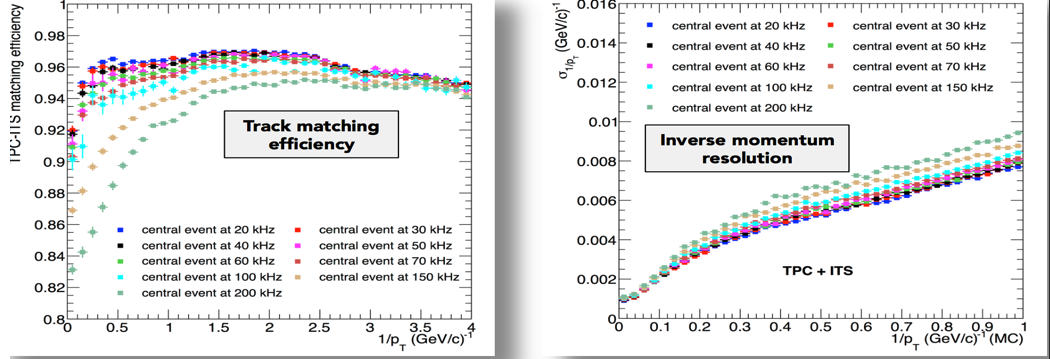
\includegraphics[width=\linewidth]{ResoSim}
\centering
\caption{ITS-TPC matching  \textit{(left)} and inverse momentum resolution \textit{(right)} for a 4-GEM stack simulated in Garfield++ \cite{Dick2017QM}. }
\label{fig:ResoSim}
\end{figure}


Figure \ref{fig:ResoSim} shows simulations of the track matching efficiency from the ITS to the TPC and the inverse momentum resolution for a 4-GEM stack as a function of several collisions.  The efficiency and resolution only start to diminish at an event rate above 100 kHz, which is double the expected rate after the LHC upgrade, and are well within the range of the current TPC, operating at 3.5 kHz.
 
\begin{figure}[h]
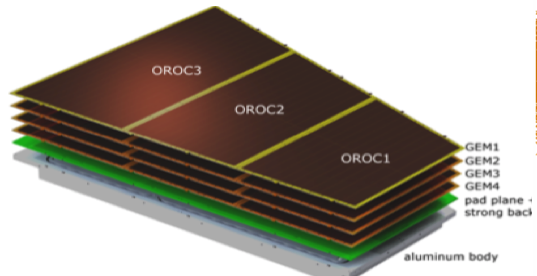
\includegraphics[width=10.0cm]{4GEMROC}
\centering
\caption{Final design of the upgraded readout chambers with a stack of 4 GEMS \cite{CERN-LHCC-2013-020}. }
\label{fig:4GEM}
\end{figure}

The optimal hole configuration was also explored with simulations.  Having a first and forth layer with a pitch of 140 $\mu m$ and the second and third layer with a pitch of 280 $\mu m$, allowed for the ROCs to maintain minimal ion back flow while amplifying the signal from tracks.  Figure \ref{fig:4GEM} shows the design of the ROCs with a 4-GEM stack.  The copper pad plane is glued to a reinforced fiberglass sheet, known as the strongback, to add material strength.

\subsubsection{2014 Test Beam}

During the 2014 test beam, I mounted the prototypes on the beam line, recorded data from the test beam, and monitored the performance in real time.  To quantify the performance of the prototype, it is useful to define the effective gain ($G_{eff}$) and ionic back flow percentage (IBF\%).  The effective gain is a measure of the amplification properties and in a gaseous detector is defined as

\begin{equation}
G_{eff}=\frac{I_{anode}}{\textit{e} \,  N_{ion} \ R}
\label{eq:gain}
\end{equation}
\noindent
where $\textit{e}$ is the fundamental electric charge of an electron, $I_{anode}$ is the current in the anode$, N_{ion}$ is the number of captured ions, and R is the illumination rate from an active source.

The IBF\% is defined as,

\begin{equation}
IBF \% = \frac{ I_{cathode} }{ I_{anode} } = \frac{1 + \epsilon }{ G_{eff} }
\label{eq:IBF}
\end{equation}

\noindent
where $ I_{cathode} / I_{anode}$ is the ratio of the currents measured in the cathode and anode portion of a readout as seen in Figure \ref{fig:TPCreadout}.  The IBF\% can also be defined in terms of the number of backflowing ions ($\epsilon$) created at an effective gain ($G_{eff}$).  

The test involved using the beam from both the SPS and PS\footnote{See Section \ref{sec:LHCop}.} at the LHC cast onto an iron target.  This iron target created secondary showers and tracks were measured by the prototype for both energy resolution and PID performance.  The nominal TPC gas of $CO_{2}-N_{2}\,$(90-10) was used during the test beam.  

\begin{figure}
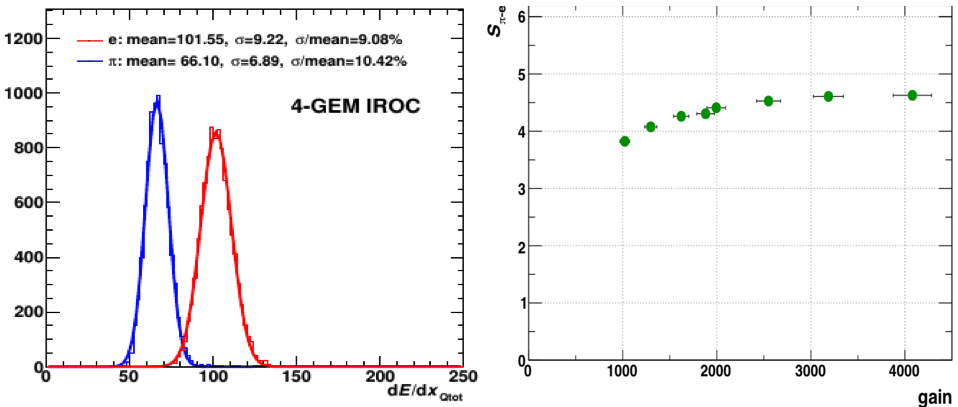
\includegraphics[width=\linewidth]{GemProtoPID}
\centering
\caption{dE/dx resolution of the 4-GEM IROC prototype\textit{(left)} and the separation power between electrons and pions as a function of gain \textit{(right)}\cite{CERN-LHCC-2015-002}.}\
\label{fig:GemProtoPID}
\end{figure}


Figure \ref{fig:GemProtoPID} shows the particle identification performance for separating electron and pion tracks created by the iron target.  The separation power between the two Gaussian peaks increases until a gain of 2000 so this was chosen as the target effective gain for the new ROCs.

\begin{figure}[h]
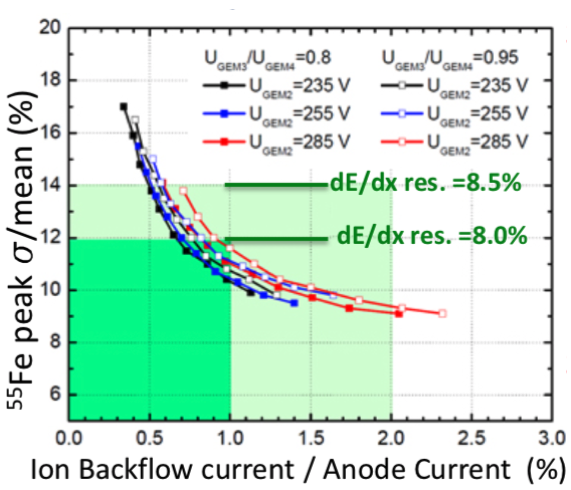
\includegraphics[width=7.0cm]{ProtoIBFEres}
\centering
\caption{Energy resolution of the iron peak as measured from the prototype IROC with varying GEM voltages as a function of IBF\%\cite{CERN-LHCC-2015-002}.}
\label{fig:ProtoIBFEres}
\end{figure}

Figure \ref{fig:ProtoIBFEres} shows the energy resolution of the iron peak as a function of the relative voltages between GEM 2 ($U_{GEM2}$) and the ratio of voltages between GEM 3 ($U_{GEM3}$) and GEM 4 ($U_{GEM4}$).  This shows that the IBF\% remains below 1\% at an energy resolution of approximately 10\% which is consistent with the current TPC performance.  The voltages were chosen such that GEM 1 and GEM2, which are closest to the drift volume, would focus mostly on capturing backflow ions, while GEM 3 and GEM 4, which are closest to the copper pad readout, would primarily perform the amplification as shown in Figure \ref{fig:showersim}.

\begin{figure}[h]
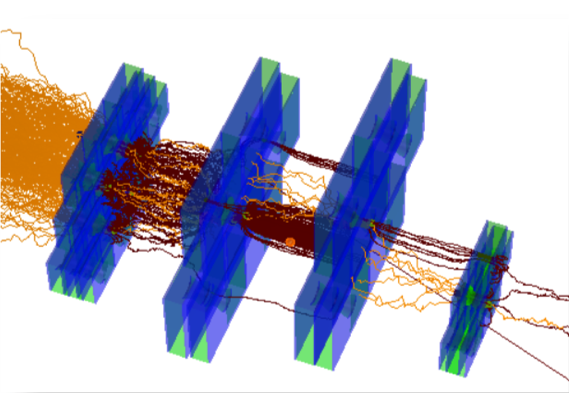
\includegraphics[width=8.0cm]{GEMShowerSim}
\centering
\caption{Simulation of the four GEM (blue) layers after test beam.  The configuration is such that the two GEMs closest to the drift volume (right) absorb the amplification ions created by the two GEMs closest to the readout (left) \cite{CERN-LHCC-2015-002}.}
\label{fig:showersim}
\end{figure}

\section{Production of The Inner Readout Chambers}

Once a final design was settled on from the simulation and prototype R\&D, the project entered the production phase.  A minimum of 36 new ROCs needed to be built with the 4-GEM stack to replace the old ROCs in the TPC, while 4 additional ROCs were constructed as spares.  Due to the size and weight of the ROCs, production of the IROCs took place in the United States and the OROC production mainly in Germany. 

\afterpage{%
\begin{figure}[h]
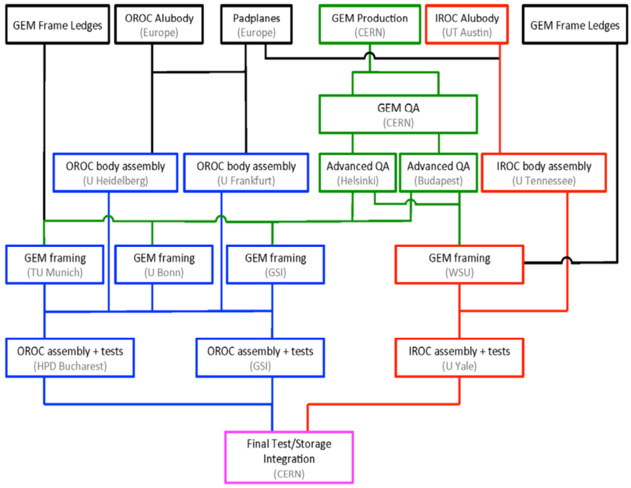
\includegraphics[width=\linewidth]{IROCproductionflow}
\centering
\caption{Production flow of the IROCs (red), OROCs (blue), and GEM foils (green)\cite{Dick2017QM}. }
\label{fig:IROCprod}
\end{figure}
\clearpage
}


Figure \ref{fig:IROCprod} shows the production flow for the construction of the 4-GEM ROCs.  After GEMs were received from the manufacturer, they went through a number of quality assurance tests before they were shipped to Wayne State University, where they were stretched and mounted for the IROCs.   The aluminum bodies were manufactured at the University of Texas Austin and shipped to Tennessee.  At Tennessee we glued the pad plane, aluminum body and strong back together before it was shipped to Yale, where the chambers were fit with the GEMs from Wayne State.  The production steps for the OROC mirror those performed by the IROC except that it was performed mainly by German institutes.

\begin{figure}[h!]
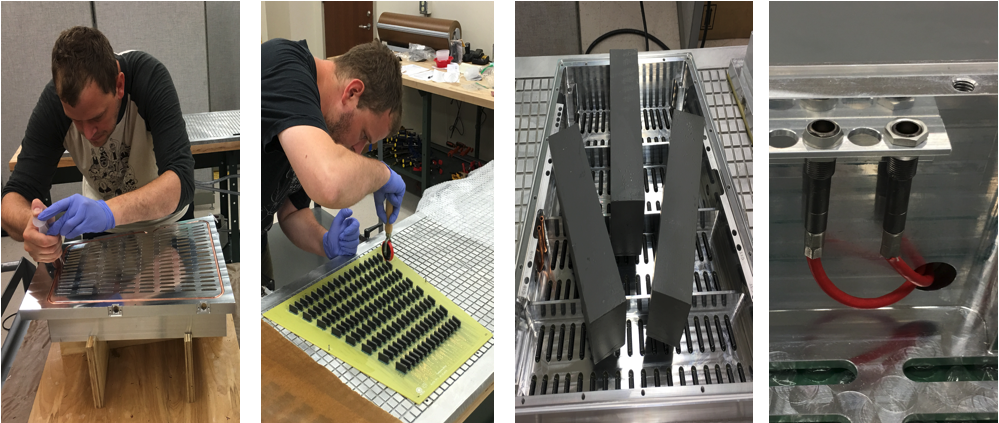
\includegraphics[width=\linewidth]{IROCAssemblyUTK}
\centering
\caption{The author assembling an Inner Readout Chamber at Tennessee. }
\label{fig:IROCassm}
\end{figure}

Figure \ref{fig:IROCassm} shows the procedure followed at Tennessee in order to build an IROC.  Furthest on the left is a picture of a copper pipe glued into the aluminum body.  This copper pipe is flushed with a coolant that maintains the temperature of the Front End Electronics (FEE) during data taking.  The next two photos show the pad plane being mounted on a vacuum table while glue is applied to it and the aluminum body.  Once all the components were placed, glued, and mounted on the table the IROC was loaded with lead bricks and allowed to cure for 24 hours.  The right most picture shows the final step of the high-voltage (HV) feedthroughs mounted and glued for the GEM foils.  Before a completed IROC left Tennessee we performed a gas tightness test that will be discussed more in the next section.  Full production of the IROCs ended in November of 2018 with a total of 49 chambers being built at Tennessee.  Eight surplus of chambers were built with excess materials to provide spares.

\section{GEM and Chamber Quality Assurance}

A stringent set of quality assurance (QA)\cite{Brucken:2018rej}\cite{Brucken:2017qjy} protocols were implemented to monitor any damage sustained during transport and to quickly identify any flaws in the production procedures.  The QA can be broken into two major categories: QA performed on the GEM foils as received from the manufacturer and QA performed on complete/semi-complete chambers as they were going through the different production steps.  I will discuss only the QA tasks that I was directly involved with.

\subsubsection{GEM Quality Assurance}

In order to evaluate the performance of a GEM foil, a spark test was performed on every foil.  Sparks are caused by the discharge of the foil and may be due to the presence of dust on a foil, imperfections in the hole geometry, or a short between the two copper layers of the GEM.  The final design of the GEM foil segmented each into twelve sectors with a 10$\: M \Omega$ bias resistor to ground across every segment.  Any sparks from charge accumulation that occur on the GEM will only discharge a given segment and not the entire foil.  Because of the delicate nature of the GEM foil, sparks have the potential to permanently damage a foil or seriously effect the performance of a ROC.  Thus GEMs with a high spark rate should be excluded as soon as possible in the production flow.

\begin{figure}[h]
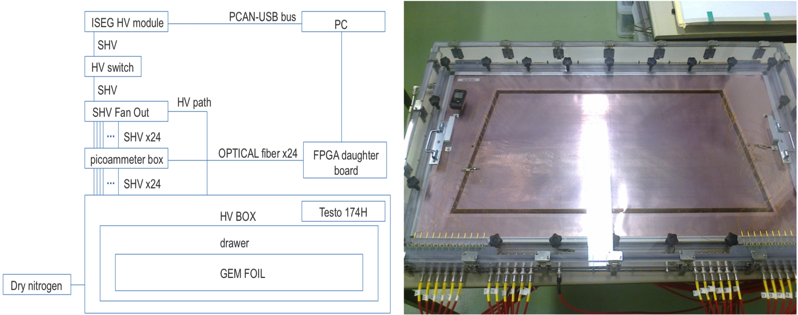
\includegraphics[width=\linewidth]{PicoSetup}
\centering
\caption{Schematic for the setup of the GEM foil spark test (\textit{left})\cite{Brucken:2018rej} and the GEM mounted in the HV gas box (\textit{right}). }
\label{fig:PicoSetup}
\end{figure}


The GEM foil spark test involved mounting each foil in a high voltage box, which was flushed with $N_{2}$ until it reached a relative humidity of $\approx 10\%$.  Once this humidity was reached 500 V is placed across each segment of the GEM and and monitored with a LabView interface.  A spark is defined as the LabView recording a current above 10 nA across the bias resistor through any GEM segment and read by a multi-channel picoammeter.  The criteria for a GEM to fail this QA was to have more than five sparks over a 20 minute recording window.

\subsubsection{Chamber Quality Assurance}

Most of the QA I helped with was on ROC chambers as they went through the production steps.  Before completed IROC chambers were sent to Yale, I performed a gas leak test.  The leak test consisted of mounting an individual chamber into an aluminum test vessel and flushing the inside of the vessel with $N_{2}$ gas.  By using a flowmeter to measure the rate that $N_{2}$ gas entered the test vessel and an oxygen sensor to measure the amount of oxygen present at the output of the test vessel, we could infer the leak rate of each IROC chamber.  Figure \ref{fig:LeakTest} shows a schematic of the setup on the left, and a typical output from the LabView interface on the right.  By flowing at two different rates and measuring the oxygen content at each rate we could confirm the leak rate.

\begin{figure}[h]
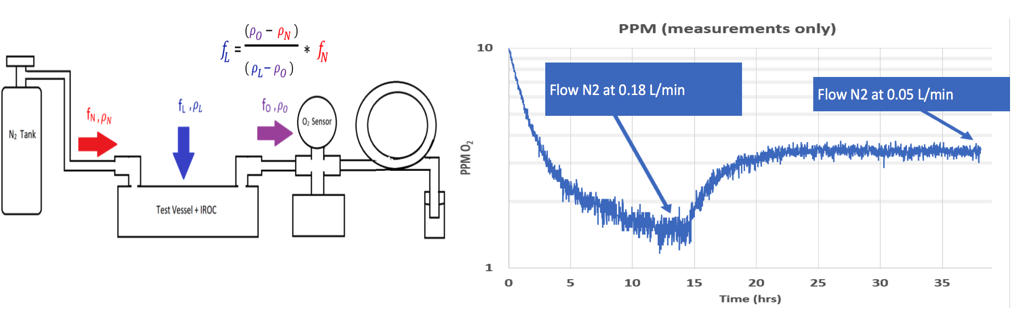
\includegraphics[width=\linewidth]{LeakSetupUTK}
\centering
\caption{Schematic of the gas tightness testing setup at the University of Tennessee \textit{(Courtesy of Joseph Rasson)}. }
\label{fig:LeakTest}
\end{figure}


The leak rate of a chamber, $\mathit{f_{L}}$,  can be quantified as
\begin{equation}
\mathit{f_{L}} =\Bigg(  \frac{\rho_{0} -\rho_{N}}{\rho_{L} -\rho_{0}} \Bigg) \,  \mathit{f_{N}}
\label{eq:leakrate}
\end{equation}

\noindent
where $\mathit{f_{N}}$ is the flow rate of $N_{2}$ gas into the test vessel, $\rho_{L}$ is the concentration of $O_{2}$ in the laboratory, $\rho_{N}$ is the $O_{2}$ impurity present in the $N_{2}$ bottle, and $\rho_{0}$ is the $O_{2}$ reading from the LabView interface.  

\begin{figure}[h]
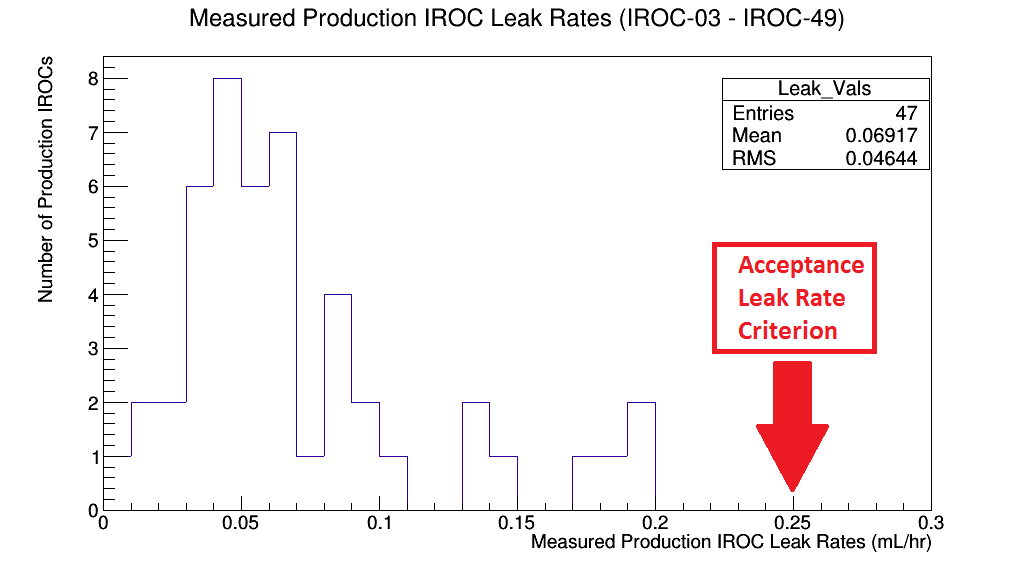
\includegraphics[width=8.0cm]{AcceptanceCriteria}
\centering
\caption{Leak rate of the 49 chambers built at Tennessee with the maximum failure rate at 0.25 ml/hr shown \textit{(Courtesy of Charles Hughes)}. }
\label{fig:IROCLeaK}
\end{figure}

\noindent
A maximum leak rate of 0.25 mL/hour was placed as the rejection criteria for a given chamber.  If a chamber had a leak rate above this, the $N_{2}$ gas could get swapped out with a helium gas tank so we could identify the areas on the IROC causing the leak with a helium sniffer and patch the area with epoxy.  Figure \ref{fig:IROCLeaK} shows the leak rate for all IROCs produced at Tennessee.  Due to none of the chambers surpassing the leak threshold the helium sniffer was not used in the production of the IROCs. 

Once an IROC chamber was fitted with the 4 GEM foils at Yale and sent to CERN, a spark test was performed over the entire chamber.  The test involved placing each chamber next to the LHC beam line, flushing with the nominal TPC gas, placing the nominal voltage across each GEM, and monitoring the spark rate once a beam was present in the LHC.   Figure \ref{fig:LHCspark} shows me installing the completed IROC chambers next to the LHC beam line in front of ALICE and the output from the spark monitor.  The voltage across each chamber could be varied in real time in order to minimize sparking while maintaining the IROC performance, thus reducing the rate of degradation on a per chamber basis once installed in the TPC.


\begin{figure}[h]
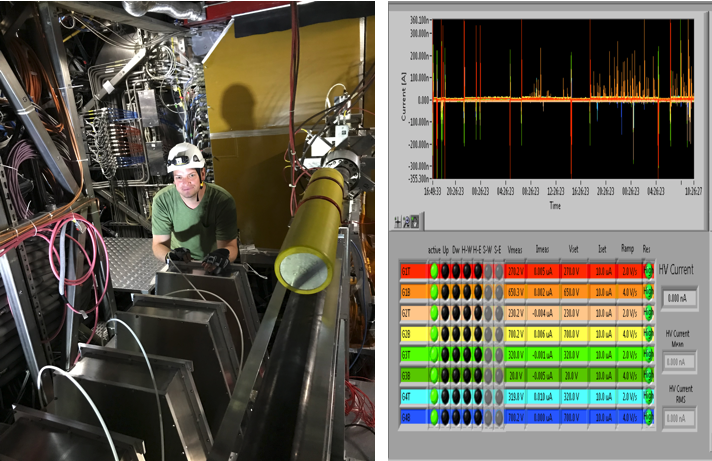
\includegraphics[width=14.0cm]{LHCSparkTest}
\centering
\caption{Testing for chamber sparking next to the LHC beam line \textit{(left)} and real time output from the spark test during a live beam (\textit{right}). }
\label{fig:LHCspark}
\end{figure}

\section{Outlook}

As of 2019, the 49 IROCs assembled at Tennessee have been received at CERN.  None of the built chambers have surpassed the gas leak test performed at CERN and so far only 4 chambers exhibit sparking rates above the failure threshold.  Due to having 13 spare IROC chambers we evaluated all the chambers for the 36 best performing IROCs for the final installation. In May of 2019, the LHC beamline around ALICE was decommissioned and the TPC was moved to a surface level clean room for the installation of the chambers.  The new FEE electronics and the ROC chambers were installed in the TPC through the summer of 2019.  Afterwards, there will be a 10 month commissioning with the TPC, during which the performance of the upgraded TPC will be evaluated with cosmic rays.  By the end of 2020, the TPC should be back in the ALICE cavern and the beam line will have been re-installed.  The Hi-Lumi run of the LHC is expected to start in March of 2021.





